%!TEX root = ../MasterThesis.tex

\chapter{Concept for a system supporting \gls{E-commerce} fraud investigations} % (fold)
\label{cha:system_concept}

This first section of the main part of the Master thesis looks into the concept  of a collaborative system that will improve the situation described in the scenario in Section~\ref{sec:scope_thesis}. Initially this chapter will discuss the overall concept of the proposed system on an high level without going to much into implementation specifics. This will answer the question of what the system is and should be able to achieve. After this initial conceptual view the chapter will further look into existing design approaches and discusses why they are of no use in this specific situation.

% sub chapter design overview
%!TEX root = ../MasterThesis.tex

\section{A data model for \gls{E-commerce} transactions}
\label{sec:data_model_transactions}

Based on the explanations in Chapter~\ref{cha:context_analysis}, and especially the scope definition for this Master thesis in Section~\ref{sec:scope_thesis}, the collaborative system for investigating \gls{E-commerce} fraud incidents have to answer the central question:\@

\begin{quotation}
  \textit{Is this transaction really a valid \gls{E-commerce} transaction?}
\end{quotation}

The relevant stakeholders, that need to be involved in the investigation process, are:\@

\begin{enumerate}
    \item \textbf{merchants}, who can provide additional information of each \gls{E-commerce} transaction in question
    \item \textbf{\gls{PSP}s/issuers}, that have information about the credit card usage patterns and the original credit card owners
    \item \textbf{\gls{LSP}s}, who can offer information about whether an order has already been shipped or not, and in the former case to whom it has been handed over
\end{enumerate}

Ideally each of those participants would make parts of their internal data structures available for the others to access and query for information. That would allow the stakeholder, who has to authorize or validate a suspicious credit card payment, to analyze all available information, as depicted in the Figure~\ref{fig:images_system_overview}.\@

\begin{figure}[H]
	\centering
		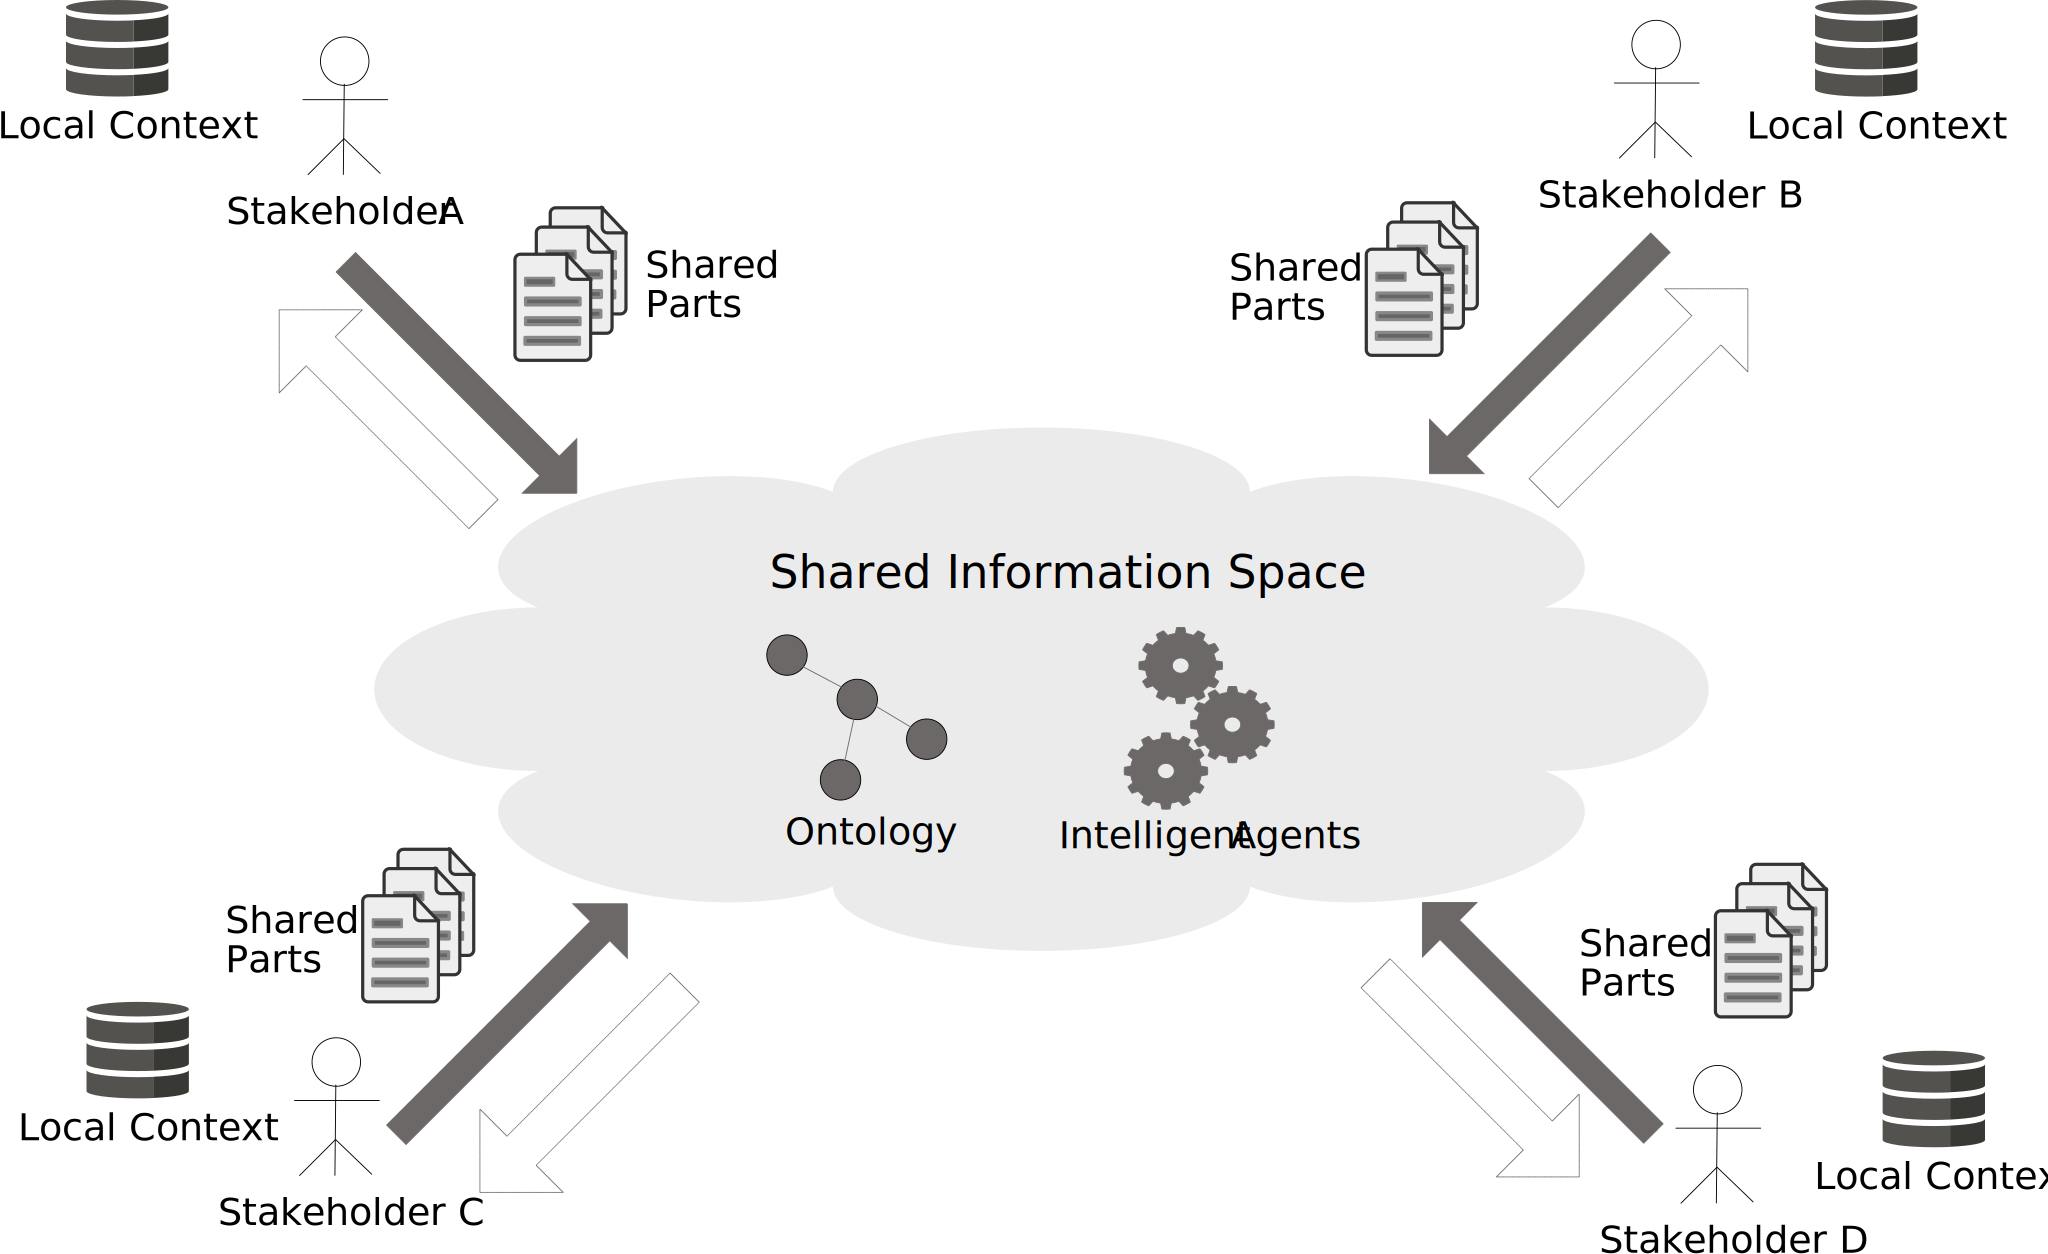
\includegraphics[width=0.9\columnwidth]{images/system_overview.pdf}
	\caption{High-level concept of the system}
\label{fig:images_system_overview}
\end{figure}

In this figure one can see that the relevant parties are providing access to parts of their internal local context information within a shared information space. Due to the fact that data from various sources have to be combined into a shared understanding of the \gls{E-commerce} activities of a consumer, there is a need to harmonize and transform the information from each participant into a shared data model to be able to analyze the combined data set. Based on this shared data model a set of intelligent agents (aka analysis algorithms) can be executed and present their findings, that can be valuable to any of the participants. \\

Based on the discussions in Chapter~\ref{cha:context_analysis}, and the analysis of the information each stakeholder holds and transmits to others, the following initial data relationships can be conducted for the \gls{E-commerce} scenario (see Figure~\ref{fig:images_data_model}). This figure shows not only the relevant information from the local contexts of each stakeholder, but also how they can be combined within a shared information space. \\

\begin{figure}[!ht]
  \centering
  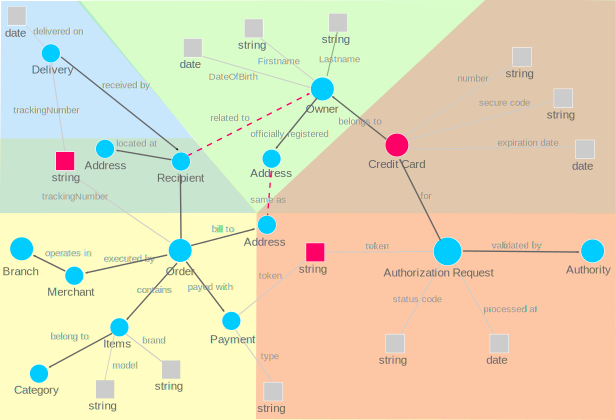
\includegraphics[width=0.9\columnwidth]{images/ontology_scenario_1.pdf}
  \caption[Data relations in the E-commerce scenario]{Data relations in the \gls{E-commerce} scenario\protect\footnotemark}
\label{fig:images_data_model}
\end{figure}

As the figure also shows there are shared information tokens between various stakeholders. Those can be used in the collaborative system as a reference for joining the distributed pieces of information into a combined view of the \gls{E-commerce} transactions. There are actually three important tokens: \@

\begin{enumerate}
  \item \textbf{payment token}: shared between merchants and \gls{PSP}s
  \item \textbf{tracking number}: shared between merchants and \gls{LSP}s
  \item \textbf{credit card}: shared between issuers and \gls{PSP}s
\end{enumerate}

In addition to these tokens the Figure~\ref{fig:images_data_model} also shows the important validation criteria. These are connections that have an influence on the decision whether an \gls{E-commerce} transaction is evaluated as suspicious or not. The two main criteria are: \@

\begin{enumerate}
  \item \textbf{billing address-to-owner address}: the billing address of the order has to match the registered address of the owner of the credit card used
  \item \textbf{recipient-to-owner}: the recipient of the delivery has to be related to the owner of the credit card
\end{enumerate}

Whereas the first criteria can be examined during the payment authorization process of an \gls{E-commerce} transaction based on the information transmitted between merchants and \gls{PSP}s or issuers, the second one is more difficult to validate (or can not be verified at all). The only check the \gls{LSP}s are able to do, before they are handing over the packaged items to the recipients, is to verify that they are the ones mentioned in the shipping address information of the order. If a recipient is somehow related to the owner of the credit card used for paying an order, or just a deceiver misusing a credit card can not be confirmed by the \gls{LSP}. \\

Also merchants, \gls{PSP}s and issuers have no possibility to check for this criteria. Whereas the merchants are able to validate whether a consumer has send items to a shipping address before, they can not restrict consumers to choose only validated recipient addresses for their orders. Doing so will have a negative impact on the business success of the online merchants. The \gls{PSP}s and issuers can not analyze this situation either, as both participants will not receive any information about the delivery address of an order with the payment authorization request from a merchant.

% section system_overview (end)


% sub chapter design overview
%!TEX root = ../MasterThesis.tex

\section{Analysis of \gls{E-commerce} transactions}
\label{sec:analyse_transactions}

Based on the explanations in the previous section the idea is to link the transaction information from various merchants, \gls{LSP}s, \gls{PSP}s and issuers together into a shared information space to be able to analyse if there are any orders that look extraordinary, and are likely not being made by the owner of the credit card to a certain extend. Due to this proposal the collaborative system will also have to use statistical evaluations and probabilities to find and rate suspicious activities. Starting with the credit card in question an issuer can query for the order details of all the transactions that have been done with the credit card online recently. To be able to do that an issuer will likely have to query the \gls{PSP}s for the payment tokens first, before asking the affected merchants for order details to any of those payment tokens. At the end each online transaction can be mapped into an \gls{ER} model like the one shown in Figure~\ref{fig:images_data_model}, building up a large graph of entities and their relationships, which has the specific credit card in the centre of it. An abbreviated sample graph of this procedure can be seen in Figure~\ref{fig:images_credit_card_graph}. \@

\begin{figure}[H]
  \centering
  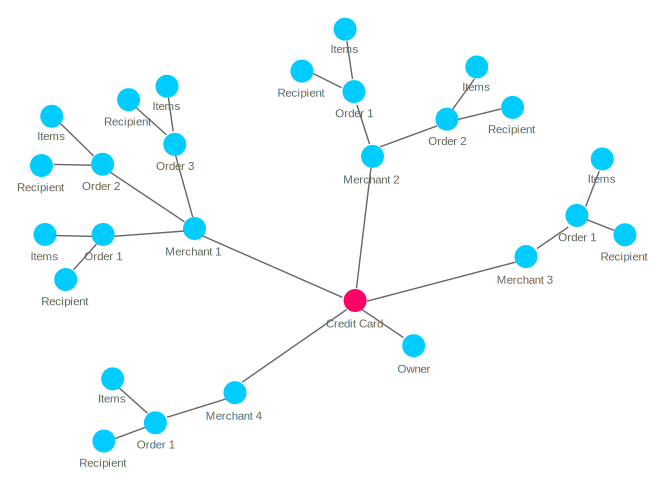
\includegraphics[width=0.9\columnwidth]{images/ontology_scenario_2.pdf}
  \caption{Building clusters of \gls{E-commerce} transactions by merchant}
\label{fig:images_credit_card_graph}
\end{figure}

As shown in this figure the transactions will be clustered by merchants first. But collecting the various order information into one combined data set is just the beginning of the \gls{E-commerce} fraud incident analysis. Based on the information received an issuer can already filter out transactions that have been shipped to different addresses than the one the credit card owner is registered for. Particularly for those edge cases it might be worth to ask for additional information from the affected merchants to be able to figure out if the consumer has used one of these shipping addresses before. As a result the existing data set can be further enriched with supplementary transactional information from merchants at any time if needed. In addition to the address information an issuer can also analyse the item information (\gls{incl}\ category, brand and model) of each order to check for malicious activities. \\

But as already stated analysing the cluster of transactions on a merchant by merchant basis will not be sufficient to come up with a solid decision about a suspicious transaction. This is mostly due to the usage pattern of the fraudsters that have been explained in the scenario in Section~\ref{sec:scope_thesis}. Based on this description the various order details from the merchants have to be mapped and linked against each other, so that the initial graph of transactions, which is clustered by merchant, can be easily transformed into complementary representations, which use different criteria to cluster the transactions such as recipient addresses, branches of merchants, or product-related information. \\

This reshaping of the transactional details can lead to new insights about the ``normal'' shopping behaviour of a credit card owner, and can make deviations from this behaviour visible. By using a clustered graph to visualize the combined data set on screen the exploratory nature of knowledge generation and perception will be supported, and so this kind of representation can help speed up the investigation of \gls{E-commerce} fraud incidents. An example visualization of a clustered graph, which groups information together based on a chosen criteria, is depicted in Figure~\ref{fig:images_graph_viz}. The different colours in this figure can represent different sources of information (e.g.\ \gls{E-commerce} transactions from various merchants). In this example information that stands out from the ``normal behaviour'' can be found in the top right and lower left areas of the figure. \@

\begin{figure}[H]
  \centering
  \includegraphics[width=0.8\columnwidth]{images/GraphViz.png}
  \caption[An example visualization of a clustered graph]{An example visualization of a clustered graph \citep{griffsgraphs}}
\label{fig:images_graph_viz}
\end{figure}

 In addition to these clustered graph visualizations the collaborative system can also support the \gls{E-commerce} fraud investigation by switching the type of representation based on the chosen criteria; e.g.\ when clustering transaction details based on location information such as shipping addresses the system can present the information as a heat map on a chart as is displayed in Figure~\ref{fig:images_map_heatmap}. \@

\begin{figure}[H]
  \centering
  \includegraphics[width=0.9\columnwidth]{images/Heatmap.png}
  \caption{Heatmap displaying clusters of location-based information}
\label{fig:images_map_heatmap}
\end{figure}

Additionally, the collaborative system can provide a Hypertext-based visualization of the linked information to allow investigators navigating through the consolidated order details done with a credit card recently. \\

To conclude the system have to support the collection and combination of \gls{E-commerce} transaction information from various sources into a linked data set using a graph-oriented data model. This graph can further be analysed from multiple view points to validate if there are any transactions that stand out from the ``normal'' shopping behaviour of the credit card owner. The starting point for the investigation is a sequence of payment tokens of recent credit card activities that an issuer can provide to the \gls{PSP}s. The linked data set will initially collect and cluster the information from each merchant based on this list. In case there are already suspicious information in one of these clusters, an issuer can ask for further details and enrich that specific cluster with additional order information for this consumer and that merchant. In the final step the system has to do the mapping and linking of the order detail information between each merchant to allow subsequent analysing and clustering of the transaction details based on various criteria.

% section system_overview (end)


% sub chapter existing approaches
\input{chapter/existing_approaches}

% chapter concept system (end)
